\documentclass[a4paper,12pt]{article}
\usepackage{tikz}
\usepackage{caption}

\usetikzlibrary{positioning}
\usetikzlibrary{shapes.geometric, arrows}
\tikzstyle{startstop} = [rectangle, rounded corners, minimum width=3cm, minimum height=1cm,text centered, draw=black, fill=red!30]
\tikzstyle{io} = [trapezium, trapezium left angle=70, trapezium right angle=110, minimum width=3cm, text width=3cm, minimum height=1cm, text centered, draw=black, fill=blue!30]
\tikzstyle{process} = [rectangle, minimum width=3cm, minimum height=1cm, text centered, text width=3cm, draw=black, fill=orange!30]
\tikzstyle{decision} = [diamond, minimum width=3cm, minimum height=1cm, text centered, draw=black, fill=green!30]
\tikzstyle{arrow} = [thick,->,>=stealth]

\begin{document}
\section*{First use case: Learning a new object}
The use case which should be implemented can be described as follows: First Hobbit should grab the turntable from its storing position. Then a message on its tablet should be shown to ask the user to put an object on the table. After the user confirmed the placement, Hobbit should look at the object on the turntable and tell the user "I'm learning a new object" via its tablet interface. The table should turn clockwise first, before the user should be asked to place the the object upside down on the table. Again, the robot should wait for confirmation, then telling "I'm learning a new object" wihle rotating the table counterclockwise. After that, the user should be asked to remove the object and confirm the action. Then Hobbit should look straight, store the table and ask for the name of the object. Finally Hobbit should show a happy emotion and tell "Thank you, now I know what \textit{X} is", where \textit{X} is the name of the object. The desired workflow is visualed in figure \ref{fig:FirstUserCaseFlow}. \\

Please implement a solution using the Blockly editor, which lets Hobbit show the desired behaviour, with respect to the following conditions:
\begin{itemize}
    \item Start working by clicking the "Start" button of the interface
    \item Do not close the graphical editor during your work
    \item Click the "Stop" button when you finished implementation
    \item Click "Submit" to submit your solution
    \item Each block provides a help page - it is accessible via \textit{right click} $\rightarrow$ \textit{Help}
\end{itemize}

\begin{figure}[!htbp]
	\centering
    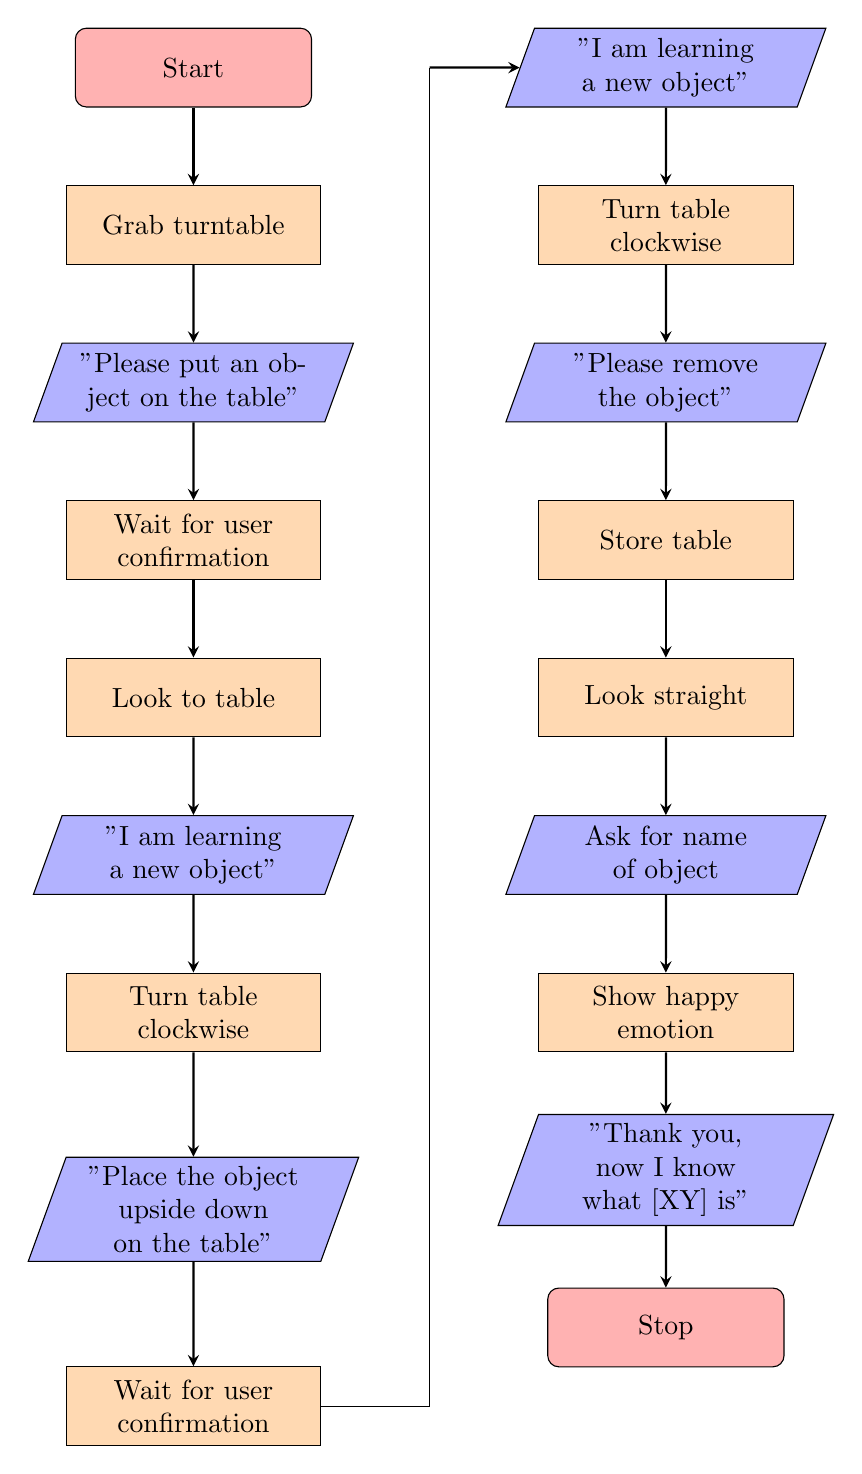
\begin{tikzpicture}[node distance=2cm]
        \node (start) [startstop] {Start};
        \node (pro1) [process, below of=start] {Grab turntable};
        \node (in1) [io, below of=pro1,] {"Please put an object on the table"};
        \node (pro2) [process, below of=in1] {Wait for user confirmation};
        \node (pro3) [process, below of=pro2] {Look to table};
        \node (out1) [io, below of=pro3] {"I am learning a new object"};
        \node (pro4) [process, below of=out1] {Turn table clockwise};
        \node (in3) [io, below of=pro4, yshift=-0.5cm] {"Place the object upside down on the table"};
        \node (pro5) [process, below of=in3, yshift=-0.5cm] {Wait for user confirmation};
        \node (out2) [io, right of=start, xshift=4cm] {"I am learning a new object"};
        \node (pro6) [process, below of=out2] {Turn table clockwise};
        \node (in4) [io, below of=pro6] {"Please remove the object"};
        \node (pro7) [process, below of=in4] {Store table};
        \node (pro8) [process, below of=pro7] {Look straight};
        \node (in5) [io, below of=pro8] {Ask for name of object};
        \node (pro9) [process, below of=in5] {Show happy emotion};
        \node (out3) [io, below of=pro9] {"Thank you, now I know what [XY] is"};
        \node (stop) [startstop, below of=out3] {Stop};
        \draw [arrow] (start) -- (pro1);
        \draw [arrow] (pro1) -- (in1);
        \draw [arrow] (in1) -- (pro2);
        \draw [arrow] (pro2) -- (pro3);
        \draw [arrow] (pro3) -- (out1);
        \draw [arrow] (out1) -- (pro4);
        \draw [arrow] (pro4) -- (in3);
        \draw [arrow] (in3) -- (pro5);
        \draw (pro5) -| (3,0);
        \draw [arrow] (3,0) -- (out2);
        \draw [arrow] (out2) -- (pro6);
        \draw [arrow] (pro6) -- (in4);
        \draw [arrow] (in4) -- (pro7);
        \draw [arrow] (pro7) -- (pro8);
        \draw [arrow] (pro8) -- (in5);
        \draw [arrow] (in5) -- (pro9);
        \draw [arrow] (pro9) -- (out3);
        \draw [arrow] (out3) -- (stop);

    \end{tikzpicture}
    \caption{Flowchart of first use case} \label{fig:FirstUserCaseFlow}
\end{figure}

\end{document}